The Low Level Dynamic~(LLD) semantics remove all the non-deterministic choices
in the previous dynamics and makes them deterministic. The new semantics will do
the following:

\begin{itemize}

   \item Match rules by priority order;

   \item Determine the set of linear facts needed to match either the rule's LHS
      or the LHS of comprehensions/aggregates without guessing;

   \item Apply as many comprehensions as the database allows.

   \item Apply as many aggregates as the database allows.

\end{itemize}

While the implementation presented in Chapter~\ref{chapter:local} follows the
LLD semantics, there are several optimizations not implemented in LLD, such as:

\begin{itemize}
   \item Indexing: the implementation uses indexing for looking up facts using a
      specific argument;
   \item Better candidate rules: when selecting a rule to execute, the
      implementation filters out rules which do not have enough facts to be
      derived;
   \item Multiple rule derivation: the LLD semantics only execute one rule at
      the time, while the implementation is able to derive a rule multiple times
      when there are no conflicting rule;
   \item Matching and substitution: in the implementation, matching is done
      implicitly using variables and comparisons, while LLD uses the $\Psi$
      context to hold substitutions.
\end{itemize}

The complete set of inference rules for the LLD semantics are presented in
Appendix~\ref{sec:lld}.

LLD is specified as an \emph{abstract machine} and is represented as a sequence
of state transitions of the form $\trans{S_1}{S_2}$. HLD had many different
proof trees for a given triplet $\Gamma; \Delta; \Phi$ because HLD allows
choices to be made during the inference rules. For instance, in HLD any rule
could be selected to be executed. In LLD there is only one state sequence
possible for a given $\Gamma; \Delta; \Phi$ since there is no guessing involved.
LLD semantics present a complete step by step mechanism that is needed to
correctly evaluate a LM program. For instance, when LLD tries to apply a rule,
it will check if there are enough facts in the database and backtrack until a
rule can be applied.

\subsection{Application}

LLD shares exactly the same inputs and outputs as HLD. The inputs correspond to
the $\Gamma$ and $\Delta$ fact contexts and the list of rules $\Phi$, while the
outputs correspond to the newly asserted facts in $\Gamma'$ and $\Delta'$ and
the retracted facts which are put in the $\Xi'$ context.

The first difference between LLD and HLD start when picking a rule to derive.
Instead of guessing, LLD treats the list of rules as a stack and picks the first
rule $R_1$ to execute (the rule with the highest priority). The remaining rules
are stored as a \emph{continuation}. If $R_1$ cannot be matched because there
are not enough facts in the database, we backtrack and use the rule continuation
to pick the next rule and so on, until one rule can be successfully applied.

The machine starts with a database $(\Gamma; \Delta)$ and a list of rules
$\Phi$. The initial state is always $\dostate{\Delta}{\Phi}{\Gamma}{\Pi}$.
We start by picking the first rule $R_1$ from $\Phi$:


\[
\trans{\dostate{\Delta}{R_1, \Phi}{\Gamma}{\Pi}}
{\appstate{\cdot}{\Delta}{\Phi}{\Pi}{\Gamma}{R}} \tag{select rule}
\]


If, after trying all the rules, there are no remaining candidate rules, the
machine enters into the $\m{next}$ state, which means that no more rules are
possible for this node and the machine should perform local computation on
another node.


\[
\trans{\dostate{\Delta}{\cdot}{\Gamma}{\Pi}}
   {\failstate{\Gamma}{\Delta}} \tag{fail}
\]


In order to try a particular rule, we either need to unfold the $\forall$
connective, by adding its variable to the $\Psi$ context, or, initiate the matching
process when reaching the $\lolli$ connective. The variables in the $\Psi$
context, which are initially assigned to an unknown value $\_$, will later be
assigned to a concrete value as the matching process goes forward.


\[
   \trans{\appstate{\Psi}{\Delta}{\Phi}{\Pi}{\Gamma}{\forall_{x : \tau}. A}}
   {\appstate{\Psi, x : \_ : \tau}{\Delta}{\Phi}{\Pi}{\Gamma}{A}}
                                                             \tag{open rule}
\]


\[
   \trans{\appstate{\Psi}{\Delta}{\Phi}{\Pi}{\Gamma}{A \lolli B}}
   {\matstateb{A \lolli B}{(\Delta; \Phi)}{\cdot}{\Gamma}{\Delta}{A}{\cdot \rightarrow
   \one}{\Psi}} \tag{init
                                                            rule}
\]



\subsection{Continuation Frames}

The most interesting aspects introduced by the LLD machine are the
\emph{continuation frame} and the \emph{continuation stack}. A continuation
frame acts as a choice point that is created during rule matching whenever we
try to match a fact expression against the database.  The frame considers all
the facts relevant to the expression given the current context $\Psi$.

The frame contains enough state to resume the matching process at the time of
its creation, therefore we can easily backtrack to the choice point and select
the next candidate fact from the database.  We keep the continuation frames in a
continuation stack for backtracking purposes. If, at some point there are no
candidate facts because the current variable assignments are not usable, we
update the top frame to try the next candidate fact. If all candidates are
exhausted, we pop the top frame and continue with the next available frame.

By using this match mechanism, we determine which facts need to be used to match
a rule.  Our LM implementation works like LLD, by iterating over the available
facts at each choice point and then committing to the rule if the matching
process succeeds. However, while the implementation only attempts to match rules
when the database has all the facts required by the rule's LHS, LLD is more
na\"{i}ve in this aspect because it tries all rules in order.


\subsection{Structure of Continuation Frames}

We have two continuation frame types, depending on the type of the candidate
facts.\footnote{All continuation frames have an implicit $\Psi$ context that
models variable assignments, including variable names, values and their
locations in the terms. This is important if we want to model variable
assignments and matchings.}

\subsubsection{Linear Continuation Frames}

There are two types of continuation frames. Linear frames use the form
$\lframe{\Delta}{\Delta''}{p(\widehat{x})}{\Omega; \Psi}{\Delta'}{\Omega'}$, where:

\begin{description}

   \item[$p(\widehat{x})$] atomic proposition that created this
      frame. The predicate for the proposition is $p$;

   \item[$\Delta$] multi-set of linear facts that are not of predicate $p$ plus
      all the other candidate facts of the predicate $p$ we have already
      tried, including a fact $p$, which is the current candidate fact;

   \item[$\Delta''$] facts of predicate $p$ that match $p(\widehat{x})$ which we
      haven't tried yet. It is a multi-set of linear facts;


   \item[$\Omega$] ordered list of remaining terms needed to match;

   \item[$\Delta'$] multi-set of linear facts we have consumed to reach this point;

   \item[$\Omega'$] terms matched already using $\Delta'$ and $\Gamma$;
   \item[$\Psi$] dictionary of variable assignments (includes variable and
      value).
\end{description}

\subsubsection{Persistent Continuation Frame}

Persistent frames are slightly different since they only need to keep track of
remaining persistent candidates. They are structured as
$\pframe{\Gamma''}{\Delta}{\bang
   p(\widehat{x})}{\Omega; \Psi}{\Delta'}{\Omega'}$:

\begin{description}
   \item[$\bang p(\widehat{x})$] persistent atomic proposition that created
      this frame;
   \item[$\Gamma''$] remaining candidate facts that match $\bang p(\widehat{x})$;
   \item[$\Delta$] multi-set of linear facts not consumed yet;

   \item[$\Omega$] ordered list of terms needed to match past this
   frame;

   \item[$\Delta'$] multi-set of linear facts consumed up-to this frame;
   \item[$\Omega'$] terms matched up-to this point using $\Delta'$ and $\Gamma$;
   \item[$\Psi$] dictionary of variable assignments (includes variable and value).
\end{description}


\subsection{Match}\label{sec:lld_body_match}

The matching state for the LLD machine uses the continuation stack to try
different combinations of facts until a match is achieved.  The state is
structured as $\matstate{A \lolli
   B}{\rulestk}{\lstack{C}}{\Gamma}{\Delta}{\Omega}{\Delta' \rightarrow
      \Omega'}$, where:

\begin{description}
   \item[$A \lolli B$] rule being matched: $A$ is the rule's LHS and $B$ the RHS;

   \item[$\rulestk$] rule continuation to be used if the current rule fails.
   Contains the original $\Delta_N$ and the rest of the rules $\Phi$;

   \item[$\lstack{C}$] ordered list of frames representing the continuation
   stack used for matching $A$;

   \item[$\Delta$] multi-set of linear facts still available to complete the
   matching process;

   \item[$\Omega$] ordered list of deconstructed RHS terms to match;

   \item[$\Delta'$] multi-set of linear facts from the original $\Delta_N$ that
   were already consumed ($\Delta', \Delta = \Delta_N$);

   \item[$\Omega'$] parts of $A$ already matched. They are in the form $P_1
   \otimes \dotsb \otimes P_n$. The idea is to use term equivalence and the fact
   that $\feq{\Omega, \Omega'}{A}$ to justify $\mz{\Gamma}{\Delta'}{A}$ when the
   matching process completes.

\end{description}

Not shown in the matching state is the context $\Psi$ that maps variables to
values. At the start of matching, the $\widehat{x}$ variables are set as
\emph{undefined}. Matching then uses facts from $\Delta$ and $\Gamma$ to match
the terms of the rule's LHS represented as $\Omega$. During the process
continuation frames are pushed into $\lstack{C}$ and if the matching process
fails, we use $\lstack{C}$ to restore the process using different candidate
facts. New facts also update the variables in the $\Psi$ context by assigning
them concrete values.

\subsubsection{Linear fact expression}

The first 2 state transitions are used when the head of $\Omega$ is a linear fact
expression $p$.

In the first transition we find $p_1$ and $\Delta''$ as facts from the database
that match $p$'s hidden and partially initialized arguments.  Context $\Delta''$
is stored in the second argument of the new continuation frame but is passed
along with $\Delta$ since the facts have not been consumed yet (just $p_1$).

The second transition deals with the case where there are no candiate facts and
thus a different machine state is used for enabling backtracking.

Note that the proposition $p_1, \Delta'' \prec p$ indicates that facts
$\Delta'', p_1$ satisfy the constraints of $p$ while $\Delta \npreceq p$
indicates that no fact in $\Delta$ satisfies $p$. Both propositions use the
omitted variable context $\Psi$ in order to replace the variables of $p$.


\begin{multline}
\transx{\matstateb{A \lolli B}{\rulestk}{\lstack{C}}{\Gamma}{\Delta, p_1,
\Delta''}{p(\widehat{x}),
   \Omega}{\Delta' \rightarrow \Omega'}{\Psi}}
{\matstateb{A \lolli B}{\rulestk}{\lframe{\Delta,
p_1}{\Delta''}{p(\widehat{x})}{\Omega; \m{extend}(\Psi, \theta)}{\Delta'}{\Omega'}, \lstack{C}}{\Gamma}{\Delta,
   \Delta''}{\Omega}{\Delta', p_1 \rightarrow \Omega' \otimes
      p(\widehat{x}\theta)}{\m{extend}(\Psi, \theta)}} \\
   \;\;\; (p_1,
   \Delta'' \prec p(\widehat{x}) \;\;\; \Delta \npreceq p(\widehat{x}))
   \tag{match p ok}
\end{multline}

\begin{align}
   \trans{\matstate{A \lolli
   B}{\rulestk}{\lstack{C}}{\Gamma}{\Delta}{p(\widehat{x}),
   \Omega}{\Delta' \rightarrow \Omega'}}
{\contstate{A \lolli B}{\rulestk}{\lstack{C}}{\Gamma}} \;\;\; (\Delta \npreceq
p(\widehat{x})) \tag{match p fail}
\end{align}


\subsubsection{Persistent fact expressions}

The next 2 state transitions are used when the head of $\Omega$ contains a
persistent fact expression $\bang p$. They are identical to the previous 2
transitions but they deal with the persistent context $\Gamma$.

\begin{align}
\trans{\matstate{A \lolli B}{\rulestk}{\lstack{C}}{\Gamma}{\Delta}{\bang p,
   \Omega}{\Delta' \rightarrow \Omega'}}
{\matstate{A \lolli B}{\rulestk}{\pframe{\Gamma''}{\Delta}{\bang
   p}{\Omega}{\Delta'}{\Omega'}, \lstack{C}}{\Gamma, p_1,
      \Gamma''}{\Delta}{\Omega}{\Delta' \rightarrow \Omega' \otimes \bang p}}
      \;\;\; (\bang p_1, \Gamma'' \prec \bang p) \tag{match \bang p ok}
\end{align}

\begin{align}
\trans{\matstate{A \lolli B}{\rulestk}{\lstack{C}}{\Gamma}{\Delta}{\bang p,
   \Omega}{\Delta' \rightarrow \Omega'}}
{\contstate{A \lolli B}{\rulestk}{\lstack{C}}{\Gamma}} \;\;\; (\Gamma \npreceq
      \bang p) \tag{match \bang p fail}
\end{align}


\subsubsection{Other expressions}

Finally, we have the transitions that deconstruct the other LHS terms and a
final transition to initiate the RHS derivation.


\begin{align}
\trans{\matstate{A \lolli B}{\rulestk}{\lstack{C}}{\Gamma}{\Delta}{\one,
   \Omega}{\Delta' \rightarrow \Omega'}}
{\matstate{A \lolli B}{\rulestk}{\lstack{C}}{\Gamma}{\Delta}{\Omega}{\Delta'
   \rightarrow \Omega'}} \tag{match $\one$}
\end{align}

\begin{align}
\trans{\matstate{A \lolli B}{\rulestk}{\lstack{C}}{\Gamma}{\Delta}{X \otimes Y,
   \Omega}{\Delta' \rightarrow \Omega'}}
{\matstate{A \lolli B}{\rulestk}{\lstack{C}}{\Gamma}{\Delta}{X, Y,
   \Omega}{\Delta' \rightarrow \Omega'}} \tag{match $\otimes$}
\end{align}

\begin{align}
\trans{\matstate{A \lolli
   B}{\rulestk}{\lstack{C}}{\Gamma}{\Delta}{\cdot}{\Delta' \rightarrow \Omega'}}
{
   \derstatex{\Gamma}{\Delta}{\Delta'}{\cdot}{\cdot}{B}
} \tag{match end}
\end{align}


\subsection{Backtracking}\label{sec:lld_match_cont}

The backtracking state of the machine reads the top of the continuation stack
$\lstack{C}$ and restores the matching process with a different candidate fact
from the continuation frame. The state is written as $\contstate{A \lolli
B}{\rulestk}{\lstack{C}}{\Gamma}$, where:

\begin{description}
   \item[$A \lolli B$] the rule being matched;
   \item[$\rulestk$] next available rules if the current rule does not match;
   the rule continuation;
   \item[$\lstack{C}$] the continuation stack for matching $A$;
\end{description}

\subsubsection{Linear continuation frames}

The next two state transitions handle linear continuation frames on the top of the
continuation stack. The first transition selects the next candidate fact $p_1$ from the
second argument of the linear frame and updates the frame. Otherwise, if we have
no more candidate facts, we pop the continuation frame and backtrack to the
remaining continuation stack.

\begin{align}
\trans{\contstate{A \lolli B}{\rulestk}{\lframe{\Delta}{p_2,
   \Delta''}{p}{\Omega}{\Delta'}{\Omega'}, \lstack{C}}{\Gamma}}
{
   \matstate{A \lolli B}{\rulestk}{\lframe{\Delta,
      p_2}{\Delta''}{p}{\Omega}{\Delta'}{\Omega'},
   \lstack{C}}{\Gamma}{\Delta}{\Omega}{\Delta', p_2 \rightarrow \Omega' \otimes p}}
   \tag{next p}
\end{align}

\begin{align}
\trans{\contstate{A \lolli
   B}{\rulestk}{\lframe{\Delta}{\cdot}{p}{\Omega}{\Delta'}{\Omega'},
      \lstack{C}}{\Gamma}}
{
   \contstate{A \lolli B}{\rulestk}{\lstack{C}}{\Gamma}} \tag{next frame}
\end{align}


\subsubsection{Persistent continuation frames}

We also have the same two kinds of inference rules for persistent continuation
frames.

\[
\infer[\cont \bang p~\m{next}]
{\cont [p_1, \Gamma'; \Delta; \bang p, \Omega; \Xi; \Lambda; \Upsilon], C; H; R; \Gamma \rightarrow \Xi'; \Delta'; \Gamma'}
{\mo \Gamma; \Delta; \Xi; \Omega; H; [\Gamma'; \Delta; \bang p, \Omega; \Xi; \Lambda; \Upsilon], C; R \rightarrow \Xi'; \Delta'; \Gamma'}
\]

\[
\infer[\cont \bang p~\m{no~more}]
{\cont [\cdot; \Delta; \bang p, \Omega; \Xi; \Lambda; \Upsilon], C; H; R; \Gamma \rightarrow \Xi'; \Delta'; \Gamma'}
{\cont C; H; R; \Gamma \rightarrow \Xi'; \Delta'; \Gamma'}
\]


\subsubsection{Empty continuation stack}

Finally, if the continuation stack is empty, we simply force execution to try
the next inference rule in $\Phi$.

\begin{align}
\trans{\contstate{A \lolli B}{(\Delta; \Phi)}{\cdot}{\Gamma}}
   {\dostate{\Delta}{\Phi}{\Gamma}{\Pi}} \tag{rule fail}
\end{align}


\subsection{Derivation}

Once the list of terms $\Omega$ of the LHS is exhausted, we derive the rule's
RHS. The derivation state simply iterates over $B$, the rule's RHS, and derives
terms into the corresponding new contexts. The state is represented as
$\derstatex{\Gamma}{\Delta}{\Xi}{\Gamma_1}{\Delta_1}{\Omega}$ with the following
meaning:

\begin{enumerate}
   \item[$\Gamma$] set of persistent facts;

   \item[$\Delta$] multi-set of remaining liner facts;

   \item[$\Xi$] multi-set of linear facts consumed up-to this point;

   \item[$\Gamma_1$] set of persistent facts derived;

   \item[$\Delta_1$] multi-set of linear facts derived;

   \item[$\Omega$] remaining terms to derive as an ordered list. We start with
   $B$ if the original rule is $A \lolli B$.

\end{enumerate}

\subsubsection{Fact templates}

When deriving either $p$ or $\bang p$ we have the following two inference rules:

\[
\infer[\done p]
{\done \Gamma ; \Delta; \Xi; \Gamma_1 ; \Delta_1; p, \Omega \rightarrow \outsem}
{\done \Gamma ; \Delta; \Xi; \Gamma_1 ; p, \Delta_1; \Omega \rightarrow \outsem}
\tab
\infer[\done \bang p]
{\done \Gamma ; \Delta ; \Xi; \Gamma_1 ; \Delta_1; \bang p, \Omega \rightarrow
   \outsem}
{\done \Gamma ; \Delta ; \Xi; \Gamma_1, p; \Delta_1; \Omega \rightarrow \outsem}
\]


\subsubsection{RHS deconstruction}

The following two inference rules deconstruct the RHS list $\Omega$ from terms
created using either $\one$ or $\otimes$.

\[
\infer[\done 1]
{\done \Gamma; \Delta; \Xi; \Gamma_1 ; \Delta_1; 1, \Omega \rightarrow \outsem}
{\done \Gamma; \Delta; \Xi; \Gamma_1 ; \Delta_1; \Omega \rightarrow \outsem}
\tab
\infer[\done \otimes]
{\done \Gamma ; \Delta; \Xi; \Gamma_1; \Delta_1; A \otimes B, \Omega \rightarrow
   \outsem}
{\done \Gamma ; \Delta; \Xi; \Gamma_1; \Delta_1; A, B, \Omega \rightarrow
   \outsem}
\]


\subsubsection{Aggregates}

We also have a transition for aggregates. The aggregate starts with a set of
values $\widehat{V}$ and an accumulator initialized as $\cdot$. The second state
initiates the matching process of the LHS $A$ of the aggregate (explained in
the next section).

\[
\infer[\done \m{agg}]
{\done \Gamma; \Delta ; \Xi; \Gamma_1; \Delta_1; \aggsz{A}{B}{C}, \Omega
   \rightarrow \outsem}
{\ma \Gamma; \Delta; \Xi; \Gamma_1; \Delta_1; \cdot; A ; \cdot; \cdot;
   \aggsz{A}{B}{C}; \Omega; \Delta; \cdot \rightarrow \outsem}
\]


\subsubsection{Successful rule}

Finally, if the ordered list $\Omega$ is exhausted, then the whole execution
process is done.  Note how the output arguments match the input arguments of the
$\done$judgment.

\begin{align}
\trans{\derstatex{\Gamma}{\Delta}{\Xi}{\Gamma_1}{\Delta_1}{\cdot}}
{\finalstate{\Xi}{\Gamma_1}{\Delta_1}} \tag{rule finished}
\end{align}


\subsection{Aggregates}

The most intricate part of the derivation process is processing comprehensions
and aggregates. For both of them, we need to perform as many derivations as the
database allows, therefore we need to deterministically check the contents of
the database until no more derivations are possible.  The matching process is
then similar to the process used for matching the body of the rule presented in
Section~\ref{sec:lld_body_match}, however we use two continuation stacks,
$\lstack{C}$ and $\lstack{P}$. In $\lstack{P}$, we put all the initial
persistent frames and in $\lstack{C}$ we put the first linear frame and then
everything else.

In order to reuse the stacks $\lstack{C}$ and $\lstack{P}$, we need to update
them by removing all the frames in $\lstack{C}$ pushed after the first linear
continuation frame.  If we tried to use those frames, we would assumed that the
linear facts used by the other frames were still in the database, but that is
not true because they have been consumed during the first application of the
comprehension.  For example, if the body is $\bang \mathtt{a(X)} \otimes
\mathtt{b(X)} \otimes \mathtt{c(X)}$ and the continuation stack has three frames
(one per fact), we cannot backtrack to the frame of $\mathtt{c(X)}$ because, at
that point, the matching process was assuming that the previous \texttt{b(X)}
linear fact was still available.  Moreover, we also need to remove the consumed
linear facts from the frames of \texttt{b(X)} and $\bang$\texttt{a(X)} in order
to make the stack fully consistent with the new database. We will see later on
how to do that.

\subsubsection{Example}

As an example, consider the following snippet of code inspired in the PageRank
program shown in Fig.~\ref{language:code:async_pagerank}:

\begin{Verbatim}[fontsize=\codesize]
update(A),
!numInbound(A, T)
   -o [sum => V | B, W, Val | !edge(A, B), neighbor-pagerank(A, B, Val),
         V = Val/float(T) | neighbor-pagerank(A, B, Val) | sum-ranks(A, V)].
\end{Verbatim}

Let's assume that the rule above was successfully matched with \code{A = 1} and
\code{T = 2} and the database contains the following facts: \code{\bang edge(1,
2)}, \code{\bang edge(1, 3)}, \code{neighbor-pagerank(1, 2, 0.5)} and
\code{neighbor-pagerank(1, 3, 0.5)}. Figure~\ref{fig:logic:backtrack} shows how
the aggregate is computed using the continuation stack. An initial frame is
created for \code{\bang edge(1, B)} which includes two \code{edge} facts and
\code{\bang edge(1, 2)} is selected to continue the process. Since \code{B = 2},
the frame for \code{neighbor-pagerank(1, 2, Val)} includes only
\code{neighbor-pagerank(1, 2, 0.5)} which completes the first application of the
aggregate and the same linear fact is re-derived using the first aggregate head.
Computation then proceeds by backtracking to the first linear frame, the frame
of \code{neighbor-pagerank(1, 2, Val)}, but there are no more available
candidates, therefore the frame is removed and the next candidate \code{\bang
edge(1, 3)} of frame \code{\bang edge(1, B)} is selected. Here, a frame is
created for \code{B = 3} with \code{neighbor-pagerank(1, 3, 0.5)} and the second
application of the aggregate is completed. The process backtracks again twice
but now there are no more candidates and the second aggregate head derives
\code{sum-ranks(1, 1.0)} because \code{V = 0.5 + 0.5}, completing the aggregate
computation.

\begin{figure}[ht]
   \begin{center}
      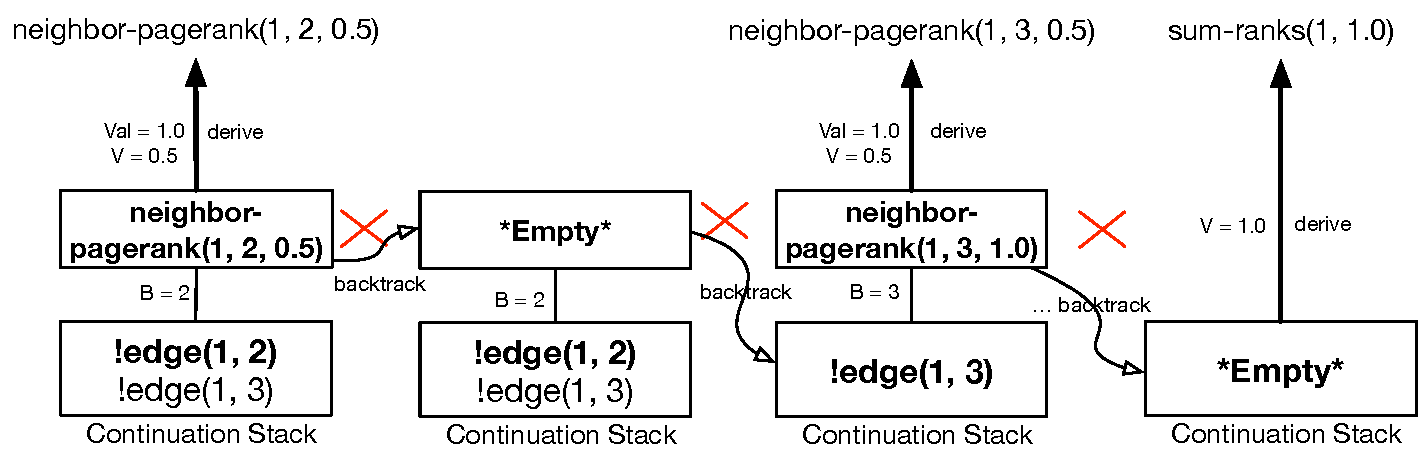
\includegraphics[width=0.85\linewidth]{figures/logical_foundations/backtrack.pdf}
   \end{center}
   \caption{Generating the PageRank aggregate.}
   \label{fig:logic:backtrack}
\end{figure}

\subsubsection{Matching}

The matching state for aggregates is 
$\matstatea{\Delta_N}{\lstack{C};
   \lstack{P}}{\Gamma}{\Delta}{\Omega}{\Delta' \rightarrow \Omega'}{\Sigma}$

\begin{enumerate}
   \item[$\Omega_N$] ordered list of remaining terms of the head of the rule to
   be derived;

   \item[$\Delta_N$] multi-set of linear facts that were still available after
   matching the body of the rule and all the previous aggregates. Note that
   $\Delta, \Xi = \Delta_N$;

   \item[$\Xi$] multi-set of linear facts used during the matching process of
   the body of the rule and all the previous aggregates;

   \item[$\Gamma_{1}$] set of persistent facts derived up to this point in the
   head of the rule;

   \item[$\Delta_{1}$] multi-set of linear facts derived up to this point in
   the head of the rule;

   \item[$\Delta'$] multi-set of linear facts consumed up to this point;

   \item[$\Omega'$] terms matched using $\Delta'$ up to this point;

   \item[$\m{agg}$] aggregate that is being matched;

   \item[$\Sigma$] the list of aggregated values;

   \item[$\lstack{C}$] continuation stack that contains both linear and persistent
   frames. The first frame must be linear;

   \item[$\lstack{P}$] initial part of the continuation stack with only persistent
   frames;

   \item[$\Delta$] multi-set of linear facts remaining up to this point in the
   matching process;

   \item[$\Omega$] ordered list of terms that need to be matched for the
   comprehension to be applied.

\end{enumerate}

Since aggregates accumulate values (from specific variables), we retrieved the
value from the $\Psi$ context. Remember that $\Psi$ is used for the
quantification connectives in the sequent calculus and in LLD is used to store
current variable bindings.

\subsubsection{Linear fact expressions}

The following two transitions deal with the case when there is a linear
fact expression in the body of the aggregate.


\begin{multline}
\transx{
   \matstatea{\deltan}{\lstack{C};
      \lstack{P}}{\Gamma}{\Delta, p_1, \Delta''}{p, \Omega}{\Delta' \rightarrow
         \Omega'}{\Sigma}
}
{
   \matstatea{\deltan}{\lframe{\Delta,
   p_1}{\Delta''}{p}{\Omega}{\Delta'}{\Omega'}, \lstack{C}; \lstack{P}}{\Gamma}{\Delta,
      \Delta''}{\Omega}{\Delta', p \rightarrow \Omega' \otimes
      p}{\Sigma}\tag{agg match p ok}
}
\end{multline}

\[
\trans{
   \matstatea{\deltan}{\lstack{C}; \lstack{P}}{\Gamma}{\Delta}{p,
      \Omega}{\Delta' \rightarrow \Omega'}{\Sigma}
}
{
   \contstatea{\deltan}{\lstack{C} ; \lstack{P}}{\Gamma}{\Sigma}
}\tag{agg match p fail}
\]


\subsubsection{Persistent fact expressions}

The transitions for dealing with persistent facts are similar to the previous
ones.



\[
\trans{
   \matstatea{\Delta_N}{\cdot;
      \lstack{P}}{\Gamma, p_1, \Gamma''}{\Delta}{\bang p, \Omega}{\Delta' \rightarrow
         \Omega'}{\Sigma}
}
{
   \matstatea{\Delta_N}{\cdot; \pframe{\Gamma''}{\Delta}{\bang
   p}{\Omega}{\Delta'}{\Omega'}, \lstack{P}}{\Gamma, p_1, \Gamma''}{\Delta}{\Omega}
   {\Delta' \rightarrow \Omega' \otimes \bang p}{\Sigma}
}
\]

\[
\trans{
   \matstatea{\Delta_N}{\lstack{C};
      \lstack{P}}{\Gamma, p_1, \Gamma''}{\Delta}{\bang p, \Omega}{\Delta' \rightarrow
         \Omega'}{\Sigma}
}
{
   \matstatea{\Delta_N}{\pframe{\Gamma''}{\Delta}{\bang
   p}{\Omega}{\Delta'}{\Omega'}, \lstack{C} ; \lstack{P}}{\Gamma, p_1, \Gamma''}{\Delta}{\Omega}
   {\Delta' \rightarrow \Omega' \otimes \bang p}{\Sigma}
}
\]


\[
\trans{
   \matstatea{\Delta_N}{\lstack{C}; \lstack{P}}{\Gamma}{\Delta}{\bang p,
      \Omega}{\Delta' \rightarrow \Omega'}{\Sigma}
}
{
   \contstatea{\Delta_N}{\lstack{C} ; \lstack{P}}{\Gamma}{\Sigma}
}
\]



\subsubsection{Deconstruct body}


\begin{multline}
\transx{
   \matstatea{\deltan}{\lstack{C};
      \lstack{P}}{\Gamma}{\Delta}{X \otimes Y, \Omega}{\Delta' \rightarrow
         \Omega'}{\Sigma}
}
{
   \matstatea{\deltan}{\lstack{C};
      \lstack{P}}{\Gamma}{\Delta}{X, Y, \Omega}{\Delta' \rightarrow
         \Omega'}{\Sigma}
} \tag{agg match $\otimes$}
\end{multline}

\begin{multline}
\transx{
   \matstatea{\deltan}{\lstack{C};
      \lstack{P}}{\Gamma}{\Delta}{\one, \Omega}{\Delta' \rightarrow
         \Omega'}{\Sigma}
}
{
   \matstatea{\deltan}{\lstack{C};
      \lstack{P}}{\Gamma}{\Delta}{\Omega}{\Delta' \rightarrow
         \Omega'}{\Sigma}
      } \tag{agg match $\one$}
\end{multline}



\subsubsection{Successful match}

When the aggregate body finally matches, we retrieve the term for variable $x$
(the aggregate variable) and add it to the list $\Sigma$.

\[
\infer[\ma{AG} \m{end}]
{\ma{AG} \Psi; \Gamma; \Delta; \Xi_N; \Gamma_{N1}; \Delta_{N1}; \Xi; \cdot;
   \lstack{C}; \lstack{P}; \Omega_N; \Delta_N; \Sigma \rightarrow \outsem}
{\fixa{AG} \Gamma; \Xi_N; \Gamma_{N1}; \Delta_{N1}; \Xi; \lstack{C}; \lstack{P}; \Omega_N;
   \Delta_N; V :: \Sigma \rightarrow \outsem & x : V : \tau \in \Psi}
\]


\subsubsection{Continuation stack update}

As we said before, to update the continuation stacks, we need remove to all the
frames except the first linear frame and remove the consumed linear facts from
the remaining frames so that they are still valid for the next application of
the aggregate.  The judgment that updates the stack has the form
$\fixstatea{\Delta}{\Xi; \Delta'}{\lstack{C};
   \lstack{P}}{\Gamma}{\Sigma}$, where:

\begin{enumerate}
   \item[$\Omega_N$] ordered list of remaining terms of the head of the rule to
   be derived;
   \item[$\Delta$] multi-set of linear facts that were still available after
   matching the body of the rule and the body of the aggregate;
   \item[$\Xi$] multi-set of linear facts used during the matching process of
   the body of the rule and all the previous aggregates;
   \item[$\Delta'$] multi-set of linear facts consumed by the aggregate body;
   \item[$\Gamma_{1}$] set of persistent facts derived by the head of the rule
   and all the previous aggregates;
   \item[$\Delta_{1}$] multi-set of linear facts derived by the head of the
   rule and all the previous aggregates;
   \item[$\m{agg}$] the current aggregate;
   \item[$\Sigma$] list of accumulated values;
   \item[$\lstack{C}, \lstack{P}$] continuation stacks for the comprehension;
   \item[$\Gamma$] set of usable persistent facts.
\end{enumerate}

\subsubsection{Remove linear continuation frames}

To remove all linear continuation frames except the first one, we simply go
through all the frames in the stack $\lstack{C}$ until only one frame remains.
This last frame and stack $\lstack{P}$ are then updated by removing $\Delta'$
from its contexts.


{\tiny
\[
\infer[\fixa ~\m{end~linear}]
{\fixa \Gamma; \Xi_N; \Gamma_{N1}; \Delta_{N1}; \Xi; (\Delta_x; \Delta''; \cdot;
      p; \Omega; \cdot; \Upsilon); P;  \aggsz{A}{B}{C}; \Omega_N; \Delta_N; T \rightarrow \Xi'; \Delta'; \Gamma'}
{\begin{split}\strans &\Xi; P; P' \\ \da \Gamma; \Xi_N, \Xi; \Gamma_{N1};
   \Delta_{N1}; B; (\Delta_x - \Xi; \Delta'' - \Xi; \cdot;& p; \Omega; \cdot;
         \Upsilon) ; P' ; \aggsz{A}{B}{C}; \Omega_N; (\Delta_N - \Xi); T &\rightarrow \Xi'; \Delta'; \Gamma'\end{split}}
\]
}

\[
\infer[\fixa \m{more}]
{\fixa \Gamma; \Xi_N; \Gamma_{N1}; \Delta_{N1}; \Xi; \_, X, C; P; AG; \Omega_N; \Delta_N; T \rightarrow \Xi'; \Delta'; \Gamma'}
{\fixa \Gamma; \Xi_N; \Gamma_{N1}; \Delta_{N1}; \Xi; X, C; P; AG; \Omega_N; \Delta_N; T \rightarrow \Xi'; \Delta'; \Gamma'}
\]

{\footnotesize
\[
\infer[\fixa \m{end~empty}]
{\fixa \Gamma; \Xi_N; \Gamma_{N1}; \Delta_{N1}; \Xi; \cdot; P; \aggsz{A}{B}{C}; \Omega_N; \Delta_N; T \rightarrow \Xi'; \Delta'; \Gamma'}
{\begin{split}\strans &\Xi; P; P' \\ \da \Gamma; \Xi_N, \Xi; \Gamma_{N1};
   \Delta_{N1}; B; \cdot ; P' ; &\aggsz{A}{B}{C}; \Omega_N; (\Delta_N - \Xi); T &\rightarrow \Xi'; \Delta'; \Gamma'\end{split}}
\]
}


\subsubsection{Aggregate backtracking}

If the aggregate match fails, we need to backtrack to the next candidate fact.
The backtracking state 
has the form
$\contstatea{\Delta_N}{\lstack{C} ; \lstack{P}}{\Gamma}{\Sigma}$, where:

\begin{enumerate}
   \item[$\Omega_N$] ordered list of remaining terms of the head of the rule to
   be derived;
   \item[$\Delta_N$] multi-set of linear facts that were still available after
   matching the body of the rule and the body of the aggregate;
   \item[$\Xi$] multi-set of linear facts used during the matching process of
   the body of the rule and all the previous aggregates;
   \item[$\Gamma_{1}$] set of persistent facts derived by the head of the rule
   and all the previous aggregates;
   \item[$\Delta_{1}$] multi-set of linear facts derived by the head of the
   rule and all the previous aggregates;
   \item[$\m{agg}$] the current aggregate;
   \item[$\Sigma$] list of accumulated values.
   \item[$\lstack{C}, \lstack{P}$] continuation stacks for the comprehension;
   \item[$\Gamma$] set of usable persistent facts.
\end{enumerate}

\paragraph{Using the $\lstack{C}$ stack}

The following 4 state transitions use the $\lstack{C}$ stack, the stack where the
first continuation frame is linear, to perform backtracking.


\begin{multline}
\transx{
   \contstatea{\deltan}{\lframe{\Delta}{p_1, \Delta''}{p}{\Omega}{\Delta'}{\Omega'}, \lstack{C} ; \lstack{P}}{\Gamma}{\Sigma}
}
{
   \matstatea{\deltan}{\lframe{\Delta,
      p_1}{\Delta''}{p}{\Omega}{\Delta'}{\Omega'}, \lstack{C}; \lstack{P}}{\Gamma}{\Delta}{p,
      \Omega}{\Delta', p_1 \rightarrow \Omega' \otimes p}{\Sigma}
} \tag{agg next p $\lstack{C}$}
\end{multline}

\begin{multline}
\transx{
   \contstatea{\deltan}{\pframe{p_1, \Gamma''}{\Delta}{\bang
   p}{\Omega}{\Delta'}{\Omega'}, \lstack{C} ; \lstack{P}}{\Gamma}{\Sigma}
}
{
   \matstatea{\deltan}{\pframe{\Gamma''}{\Delta}{\bang p}
      {\Omega}{\Delta'}{\Omega'}, \lstack{C}; \lstack{P}}{\Gamma}{\Delta}{p,
      \Omega}{\Delta' \rightarrow \Omega' \otimes \bang p}{\Sigma}
} \tag{agg next \bang p $\lstack{C}$}
\end{multline}

\[
\trans{
   \contstatea{\deltan}{\lframe{\Delta}{\cdot}{p}{\Omega}{\Delta'}{\Omega'}, \lstack{C} ; \lstack{P}}{\Gamma}{\Sigma}
}
{
   \contstatea{\deltan}{\lstack{C} ; \lstack{P}}{\Gamma}{\Sigma}
} \tag{agg  next frame $\lstack{C}$}
\]

\[
\trans{
   \contstatea{\deltan}{\pframe{\cdot}{\Delta}{\bang
   p}{\Omega}{\Delta'}{\Omega'}, \lstack{C} ; \lstack{P}}{\Gamma}{\Sigma}
}
{
   \contstatea{\deltan}{\lstack{C} ; \lstack{P}}{\Gamma}{\Sigma}
} \tag{agg next \bang frame $\lstack{C}$}
\]


\paragraph{Using the $\lstack{P}$ stack}

The following 2 state transitions rules use the $\lstack{P}$ stack instead, the stack where all
continuation frames are persistent.

\[
\infer[\conta{AG} \m{next}~\lstack{P}~\bang p]
{\conta{AG} \Gamma; \Delta_N; \Xi_N; \Gamma_{N1}; \Delta_{N1}; \cdot; f, \lstack{P}; \Omega_N; \Sigma \rightarrow \outsem}
{\begin{gathered}
   f = [p_1, \Gamma'; \Delta_N; \cdot; \bang p; \Omega; \cdot; \Upsilon] \\
   f' = [\Gamma'; \Delta_N; \cdot; \bang p; \Omega; \cdot; \Upsilon] \\
   \ma{AG} \Gamma; \Delta_N; \Xi_N; \Gamma_{N1}; \Delta_{N1}; \cdot; \Omega; \cdot;
      f', \lstack{P}; \Omega_N; \Delta_N; \Sigma \rightarrow \outsem
 \end{gathered}
}
\]

\[
\infer[\conta{AG} \m{next}~\lstack{P}~\m{empty}~\bang p]
{\conta{AG} \Gamma; \Delta_N; \Xi_N; \Gamma_{N1}; \Delta_{N1}; \cdot; f, \lstack{P}; \Omega_N; \Sigma
   \rightarrow \outsem}
{\begin{gathered}
   f =  [\cdot; \Delta_N; \cdot; \bang p; \Omega; \cdot; \Upsilon] \\
   \conta{AG} \Gamma; \Delta_N; \Xi_N; \Gamma_{N1}; \Delta_{N1}; \cdot; \lstack{P};
      \Omega_N; \Sigma \rightarrow \outsem
 \end{gathered}
}
\]


\paragraph{Aggregate done}

If both the $\lstack{C}$ and $\lstack{P}$ stacks are empty, backtracking is
impossible and the aggregate is done. The final head of the aggregate is then
derived along with the rest of the rule's head.

\[
\infer[\conta{\aggsz{A}{B}{C}} \m{end}]
{\conta{\aggsz{A}{B}{C}} \Gamma; \Delta_N; \Xi_N; \Gamma_{N1}; \Delta_{N1}; \cdot; \cdot;
   \Omega; \Sigma \rightarrow \outsem}
{\done \Gamma; \Delta_N; \Xi_N; \Gamma_{N1}; \Delta_{N1}; (\lambda x. C
      x)\Sigma,
   \Omega \rightarrow \outsem}
\]


\subsubsection{Aggregate Derivation}

After updating the continuation stacks, the subhead of the aggregate is derived.
The derivation state has the form
$\derstatea{\Delta}{\Xi}{\Gamma_1}{\Delta_1}{\Sigma}{\lstack{C};
   \lstack{P}}{\Omega}$, where:

\begin{enumerate}
   \item[$\Omega_N$] ordered list of remaining terms of the head of the rule to
   be derived;
   \item[$\Delta$] multi-set of remaining linear facts that can be used for
   the next aggregate applications.
   \item[$\Xi$] multi-set of linear facts consumed both by the body of the rule
   and previous aggregate applications;
   \item[$\Gamma_1$] set of persistent facts derived by the head of the rule,
   previous aggregates and current derivation;
   \item[$\Delta_1$] multi-set of linear facts derived by the head of the rule,
   previous aggregates and current derivation;
   \item[$\m{agg}$] current aggregate symbol;
   \item[$\Sigma$] accumulated list of values of the aggregate;
   \item[$\lstack{C}, \lstack{P}$] new continuation stacks;
   \item[$\Gamma$] set of persistent facts;
   \item[$\Omega$] ordered list of terms to derive.
\end{enumerate}

\[
\infer[\da{AG} p]
{\da{AG} \Gamma; \Delta_N; \Xi_N; \Gamma_1; \Delta_1; p, \Omega; \lstack{C}; \lstack{P}; \Omega_N;
   \Sigma \rightarrow \outsem}
{\da{AG} \Gamma; \Delta_N; \Xi_N; \Gamma_1; \Delta_1, p; \Omega; \lstack{C}; \lstack{P}; \Omega_N;
   \Sigma \rightarrow \outsem}
\]

\[
\infer[\da{AG} \bang p]
{\da{AG} \Gamma; \Delta_N; \Xi_N; \Gamma_1; \Delta_1; \bang p, \Omega; \lstack{C};
   \lstack{P}; \Omega_N; \Sigma \rightarrow \outsem}
{\da{AG} \Gamma; \Delta_N; \Xi_N; \Gamma_1, p; \Delta_1; \Omega; \lstack{C}; \lstack{P}; \Omega_N;
   \Sigma \rightarrow \outsem}
\]

\[
\infer[\da{AG} \otimes]
{\da{AG} \Gamma; \Delta_N; \Xi_N; \Gamma_1; \Delta_1; A \otimes B, \Omega; \lstack{C}; \lstack{P}; \Omega_N;
   \Sigma \rightarrow \outsem}
{\da{AG} \Gamma; \Delta_N; \Xi_N; \Gamma_1; \Delta_1; A, B, \Omega; \lstack{C}; \lstack{P}; \Omega_N;
   \Sigma \rightarrow \outsem}
\]

\[
\infer[\da{AG} \m{end}]
{\da{AG} \Gamma; \Delta_N; \Xi_N; \Gamma_1; \Delta_1; \cdot; \lstack{C}; \lstack{P}; \Omega_N;
   \Sigma \rightarrow \outsem}
{\conta{AG} \Gamma; \Delta_N; \Xi_N; \Gamma_1; \Delta_1; \lstack{C}; \lstack{P}; \Omega_N; \Sigma
   \rightarrow \outsem}
\]



This completes the specification of LLD.



